
\hypertarget{cv:registrarBR}{\section{Registrar Regla de negocio}} \label{sec:registrarBR}

	Esta funcionalidad le permitirá registrar una regla de negocio dentro del proyecto que se esta operando. 

		\subsection{Procedimiento}

			%Pasos de procedimiento
			\begin{enumerate}
	
			\item Oprima el botón \IURegistrar{} de la pantalla \ref{fig:GestionarBR} ''Gestionar Reglas de negocio''.
			
			\item Se mostrará la pantalla \ref{fig:registrarBR} ''Registrar Regla de Negocio''.

			%Pantalla
			\begin{figure}[H]
				\begin{center}
					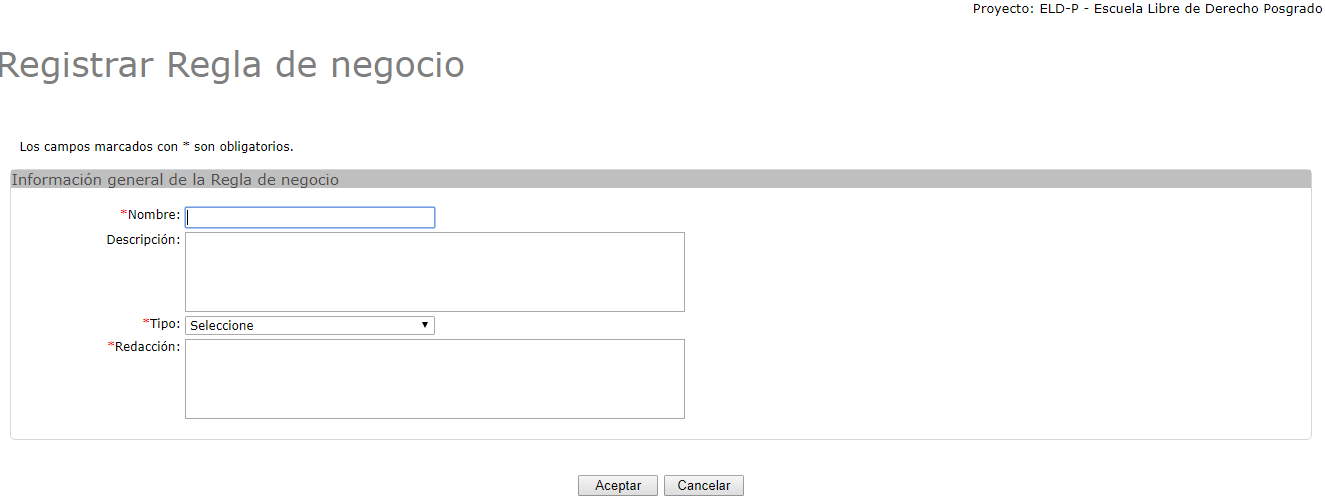
\includegraphics[scale=0.5]{roles/lider/reglasNegocio/pantallas/IU8-1registrarBR}
					\caption{Registrar Regla de Negocio}
					\label{fig:registrarBR}
				\end{center}
			\end{figure}
		
			\item Ingrese el nombre, si lo requiere una pequeña descripción de la entidad, seleccione el tipo de regla de negocio desea registrar y por último ingrese la redacción de la regla de negocio
			
			\item Dependiendo del tipo de dato que elija aparecerán nuevos campos que son requeridos para el tipo de regla de negocio seleccionado. Las siguientes pantallas muestran los campos que requiere cada tipo de regla de negocio: 
			
			\begin{figure}[H]
				\begin{center}
					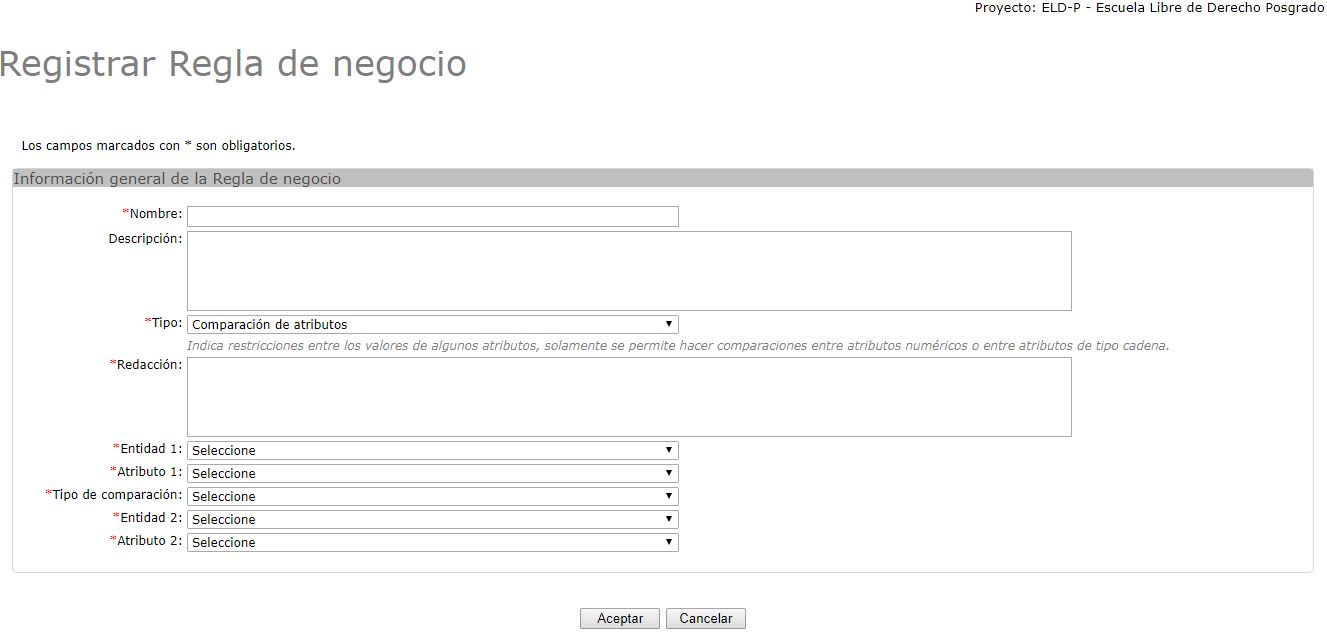
\includegraphics[scale=0.5]{roles/lider/reglasNegocio/pantallas/IU8-1AregistrarBR}
					\caption{Registrar Regla de negocio: Comparación de Atributos}
					\label{fig:registrarBRA}
				\end{center}
			\end{figure}
			
			\begin{figure}[H]
				\begin{center}
					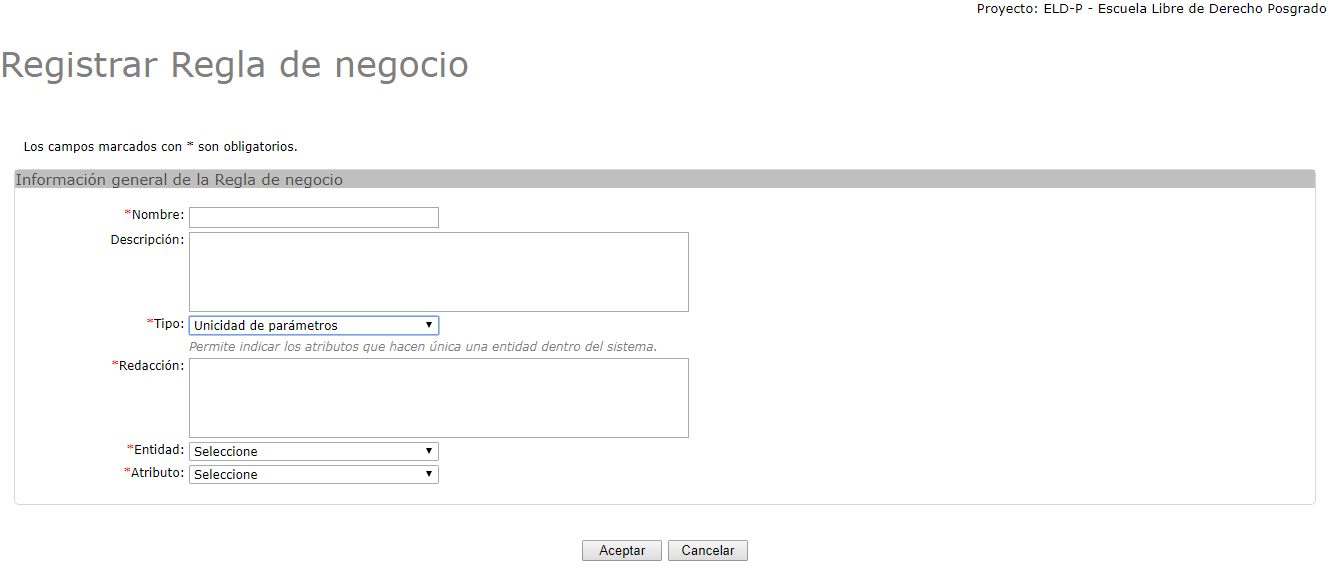
\includegraphics[scale=0.5]{roles/lider/reglasNegocio/pantallas/IU8-1BregistrarBR}
					\caption{Registrar Regla de negocio: Unicidad de parámetros}
					\label{fig:registrarBRB}
				\end{center}
			\end{figure}
			
			\begin{figure}[H]
				\begin{center}
					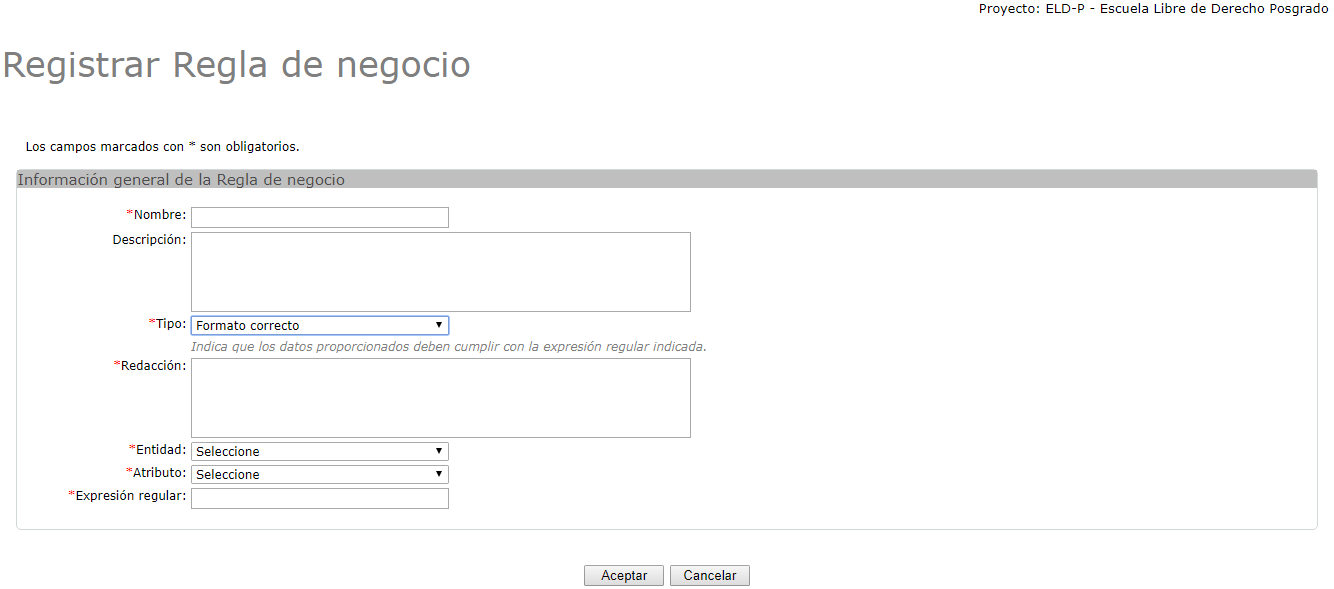
\includegraphics[scale=0.5]{roles/lider/reglasNegocio/pantallas/IU8-1CregistrarBR}
					\caption{Registrar Regla de negocio: Formato Correcto}
					\label{fig:registrarBRC}
				\end{center}
			\end{figure}
			
			\item Oprima el botón \IUAceptar.
			
			\item Se mostrará el mensaje \ref{fig:BRRegistrada} en la pantalla \ref{fig:GestionarBR} ''Gestionar Reglas de negocio''.
			
			\begin{figure}[htbp!]
				\begin{center}
					
\includegraphics[scale=0.5]{roles/lider/reglasNegocio/pantallas/IU8-1MSG1}
					\caption{MSG: Regla de Negocio Registrada}
					\label{fig:BRRegistrada}
				\end{center}
			\end{figure}
			\end{enumerate}